\documentclass[11pt]{article}
\usepackage[T1]{fontenc}
\usepackage{lmodern}
\usepackage[margin=1.05in]{geometry}
\usepackage{amsmath,amssymb,amsthm,mathtools}
\usepackage{microtype}
\usepackage{enumitem}
\usepackage{needspace}
\usepackage{tikz}
\usetikzlibrary{arrows.meta,positioning,calc,fit,backgrounds}
\usepackage[colorlinks=true,linkcolor=black,citecolor=black,urlcolor=blue]{hyperref}
\hypersetup{pdftitle={An infinite finitely presented residually finite 2-group},pdfauthor={OpenAI}}
\setlength{\emergencystretch}{2em}
\clubpenalty=10000
\widowpenalty=10000
\numberwithin{equation}{section}
\newtheorem{theorem}{Theorem}[section]
\newtheorem{proposition}[theorem]{Proposition}
\newtheorem{lemma}[theorem]{Lemma}
\newtheorem{corollary}[theorem]{Corollary}
\theoremstyle{definition}
\newtheorem{definition}[theorem]{Definition}
\theoremstyle{remark}
\newtheorem{remark}[theorem]{Remark}
\newcommand{\F}{\mathbb F}
\newcommand{\Z}{\mathbb Z}
\newcommand{\Q}{\mathbb Q}
\newcommand{\N}{\mathbb N}
\newcommand{\Id}{I}
\DeclareMathOperator{\St}{St}
\DeclareMathOperator{\E}{E}
\DeclareMathOperator{\GL}{GL}
\DeclareMathOperator{\Mat}{Mat}
\DeclareMathOperator{\Hom}{Hom}
\DeclareMathOperator{\im}{im}
\DeclareMathOperator{\rank}{rank}
\DeclareMathOperator{\supp}{supp}
\title{An infinite finitely presented residually finite 2-group}
\author{OpenAI}
\date{October 5, 2026}
\begin{document}
\maketitle
\begin{abstract}
We prove that the infinite, ordinarily finitely presented periodic
Steinberg group $\Gamma=\St_{12}(R)$ of a companion paper is residually
finite. Its finite-index subgroup
$G=\ker(\Gamma\to\St_{12}(\F_2))$ is infinite, ordinarily finitely
presented, and residually finite, and every element of $G$ has finite
$2$-power order. The orders of its elements are unbounded.
Phases of long words in the companion's graded algebra allow finite
degree truncations to detect all elements of $\Gamma$, including the
central kernel.
\end{abstract}
\section{Introduction}\label{sec:introduction}

A group is \emph{periodic} if each of its elements has finite order.
It is \emph{residually finite} if, for every nonidentity element $g$,
there is a homomorphism to a finite group whose value at $g$ is
nonidentity. We use \emph{2-group} to mean a group in which every
element has finite 2-power order; the group itself need not be finite.
An \emph{ordinary finite presentation} is a quotient of a free group
on finitely many generators by the normal closure of finitely many
words. We prove the following.

\begin{theorem}\label{thm:main}
There exists an infinite residually finite group with an ordinary finite
presentation in which every element has finite 2-power order.
\end{theorem}

The group is an abstract discrete group. Finite presentation is meant
in that category, rather than in a variety of groups or in the category
of pro-2 groups. The orders of its elements are necessarily unbounded.

\subsection*{History and relation to earlier constructions}

Burnside's finiteness questions \cite{Burnside1902} ask how finite-order
conditions constrain a group with finitely many generators. Golod's
construction \cite[Example~2]{Golod1964}, based on the
Golod--Shafarevich dimension argument \cite{GolodShafarevich1964},
already produces infinite finitely generated residually finite
$p$-groups. Its algebraic mechanism is particularly relevant here:
nilpotence gives finite $p$-power orders, while a grading separates
elements in finite quotients. Grigorchuk later gave a concrete infinite
finitely generated residually finite 2-group
\cite{Grigorchuk1980}; his original theorem also establishes that this
group is not finitely presented. Thus residual finiteness and fixed-prime
torsion can coexist with finite generation. The additional requirement
in Theorem~\ref{thm:main} is an ordinary finite presentation.

The question whether an infinite periodic group can have an ordinary
finite presentation is recorded in
\cite[p.~45]{OlshanskiiSapir2003} and again in
\cite[Section~2.2(IX)]{HaettelOsajda2025}. The torsion-by-cyclic
groups of \cite[Theorem~1.1]{OlshanskiiSapir2003} have an infinite
cyclic quotient. They establish a different finite-presentation result
and are not themselves periodic. The companion paper
\cite{Companion} constructs an infinite finitely presented periodic
group using a graded algebra with a matrix-nil positive-degree ideal.
The present paper strengthens
that construction by proving residual finiteness and passing to a
finite-index subgroup with 2-power torsion. The companion's algebra
and finite local-rule hierarchy are essential inputs; we state their
precise properties in Section~\ref{sec:ring-phases}.

A bound on all element orders would change the problem. Novikov and
Adian constructed infinite finitely generated groups of bounded exponent
\cite{NovikovAdian1968}. In the residually finite setting, however,
Zel'manov's solution of the restricted Burnside problem for 2-groups
\cite[Theorem~2]{Zelmanov1992} implies that a finitely generated
residually finite group of exponent dividing $2^a$ is finite.
Consequently the group in Theorem~\ref{thm:main} has unbounded
exponent. Its finite quotients are nevertheless all 2-groups: a finite
image has only elements of 2-power order, and Cauchy's theorem excludes
every odd prime divisor of its order.

\subsection*{The proof and its main ingredients}

The companion supplies an infinite finitely presented graded algebra
\[
 R=\F_2\oplus I,\qquad I=\bigoplus_{d\ge1}R_d,
\]
such that every matrix in $M_n(I)$ is nilpotent, for every finite $n$.
Each homogeneous component $R_d$ is finite-dimensional. The elementary
matrix group $\E_n(R)$ is generated by the matrices $e_{ij}(a)$ obtained
by adding $a\in R$ to an off-diagonal position of the identity.
The Steinberg group $\St_n(R)$ is generated by symbols $x_{ij}(a)$
subject to the elementary addition and nonopposite-root commutator
relations; these are written explicitly in
Section~\ref{sec:steinberg}. There is a natural map
\[
 \St_n(R)\longrightarrow\E_n(R),\qquad
 x_{ij}(a)\longmapsto e_{ij}(a).
\]
Finite presentability of Steinberg groups in rank at least four over
finitely presented unital rings is due to Krsti\'c and McCool
\cite[Theorem~3]{KrsticMcCool}; an adapted proof is also given in
\cite[Theorem~4.1]{Companion}. We take $n=12$ and eventually use
the kernel of reduction from $\St_{12}(R)$ to $\St_{12}(\F_2)$.

The degree truncations $R/R_{\ge d}$, where
$R_{\ge d}=\bigoplus_{b\ge d}R_b$, are finite rings. They immediately
detect nonidentity matrices over $R$. The main difficulty is to detect
elements of the Steinberg kernel as well. We first work in the stable
group $\St(R)=\varinjlim_n\St_n(R)$, put
$\E(R)=\varinjlim_n\E_n(R)$, and write
\[
 J(R)=\ker\bigl(\St(R)\longrightarrow\E(R)\bigr).
\]
This kernel is central. We first prove detection in the stable group,
where a finite calculation may always use additional coordinates.
We return to fixed rank afterward.

Two calculations of one cyclic substitution provide the detection
argument. If $z\in J(R)$, the grading replaces each homogeneous root
entry $a\in R_d$ by $at^d$. Substituting the cyclic shift matrix $C_L$
for $t$ and expanding into ordinary roots gives an element
$W_z(C_L)\in J(R)$. This is a matrix realization of a graded transfer.
Weibel's work on graded rings \cite{Weibel1987} develops the
corresponding transfer operations and their eventual vanishing; it also
implies $p$-primary torsion in relative graded $K$-groups in
characteristic $p$. Following the elementary Steinberg treatment in
\cite{Companion}, Section~\ref{sec:shifts} proves directly that
\[
 W_z(C_L)=1\quad\text{for all sufficiently large }L
\]
whenever $z$ reduces to $1$ over $\F_2$. Taking $L$ to be a power of
two also shows that every such $z$ has 2-power order.

The second calculation uses additional structure of this particular
ring. Its finite local rules give a basis of nonzero word classes.
For arbitrarily large odd integers $L$, each sufficiently long nonzero
word has a start phase $\sigma(w)\in\Z/L$ and an end phase
$\tau(w)=\sigma(w)+|w|$. These phases depend only on the word class,
and a nonzero product must match end phase to start phase.
Section~\ref{sec:ring-phases} derives the phases from the hierarchy's
bounded token decompositions.

If $z$ is missed by all degree truncations, it can be represented using
roots whose entries are arbitrarily long words. The phases allow us
to move the endpoints of each such root to coordinates labeled by its
start and end phases, without changing $z$. Establishing this identity
requires control of opposite-root commutators in the Steinberg group,
as well as a subgroup on which the matrix map is injective.
Sections~\ref{sec:long-entries} and \ref{sec:detection} prove these
facts and obtain, for the long-entry representative,
\[
 W_z(C_L)=z^L.
\]
We first choose an odd $L$ for which the first calculation vanishes,
and then find a representative long enough for the second calculation.
Thus $z^L=1$. Since $z$ also has 2-power order, it is the identity.
This proves separation by finite degree truncations, the additional
step beyond torsion supplied by graded transfers alone.

To pass back to twelve coordinates, we need the injectivity of
$\St_{12}(R)\to\St(R)$. Stability over the local ring $R$ is
covered by the classical theorem of Suslin and Tulenbaev
\cite{SuslinTulenbaev1976}. Section~\ref{sec:stability} gives a
direct integral homology proof using ordered frames and universal
central extensions of their stabilizers. This supplies the bridge
from stable detection to the finitely presented group.

All arguments establishing these phase, stabilization, and detection
claims are included below. We quote from the companion the algebra
construction and the finite-rank elementary facts needed to apply them,
with their hypotheses stated at the points of use. The final passage
to finite groups and to the subgroup of 2-power torsion is carried out
in Section~\ref{sec:construction}.

\section{The algebra and phases of long words}\label{sec:ring-phases}

The ring used below has two relevant features.  Its positive-degree
matrices are nilpotent, which will give torsion, and its long nonzero
words carry compatible positions modulo arbitrarily large odd integers,
which will give detection by finite quotients.  The first feature is an
input from the companion paper.  We derive the second from the word
hierarchy in that paper.

An ideal $I$ of a unital associative algebra is \emph{matrix-nil} if
every square matrix of every finite size with entries in $I$ is
nilpotent.  All algebras in this paper are over $\F_2$.

\begin{proposition}[The companion algebra]\label{prop:ring-input}
There is an infinite finitely presented unital associative algebra
\[
 R=\bigoplus_{d\geq0}R_d=\F_2\oplus I,
 \qquad R_0=\F_2,
 \qquad I=\bigoplus_{d\geq1}R_d,
\]
such that every $R_d$ is finite-dimensional and $I$ is matrix-nil.
This algebra has the word presentation and hierarchy specified in
Proposition~\ref{prop:hierarchy-input}.
\end{proposition}

This is the algebra constructed in \cite[Theorem~3.7]{Companion}.
We now give the precise part of its structure that we use.  In a
presentation by words, a \emph{replacement} is a relation $v=v'$
between nonempty words of equal length, usable in either direction
inside any word.  A \emph{zero declaration} is a relation $v=0$ for a
nonempty word $v$.  The length of a replacement is the common length
of its two sides.  For a word $w$, write $|w|$ for its length and $[w]$
for its image in the relevant algebra.

\begin{proposition}[The companion hierarchy]\label{prop:hierarchy-input}
The algebra $R$ in Proposition~\ref{prop:ring-input} is the first
algebra $A_0$ of a sequence $(A_j)_{j\geq0}$ with the following
properties.  There are positive integers $c,k,h_0,D$, with
$D>10(c+1)(k+1)$, and
\[
 h_j=h_0D^j,\qquad L_j=2\cdot2^{h_j}+1.
\]
For each $j\geq0$:
\begin{enumerate}[label=\textup{(\roman*)},leftmargin=*]
\item
$A_j$ is presented by a finite alphabet $\Sigma_j$, finitely many
replacements, and finitely many zero declarations, all of length at
most $k$.  It is graded by word length.
\item
There is a substitution $E_j$ sending each letter of $\Sigma_{j+1}$
to a word of length $L_j$ over $\Sigma_j$.  Extended by concatenation,
it induces a unital algebra homomorphism $A_{j+1}\to A_j$.
\item
A specified subset of $\Sigma_j$ gives cuts immediately before its
letters.  There are integers $B_j,T_j\geq0$ and a finite set of words
$\mathcal T_j$ such that every nonzero word $w$ of length at least
$T_j$ has the unique decomposition
\begin{equation}\label{eq:token-decomposition}
 w=p_w\,t_1\cdots t_r\,s_w,
 \qquad |p_w|,|s_w|\leq B_j,\qquad t_i\in\mathcal T_j.
\end{equation}
Here $p_w$ precedes the first cut, $s_w$ begins at the last cut, and
the $t_i$ are exactly the intervals between consecutive cuts.  A cut
is counted only if its following letter occurs in the word.
For each $t\in\mathcal T_j$ there is a nonempty word $u_t$ over
$\Sigma_{j+1}$ such that
\begin{equation}\label{eq:token-upper-word}
 1\leq |u_t|\leq k,\qquad
 |t|=L_j|u_t|,\qquad [t]=[E_j(u_t)]\quad\hbox{in }A_j.
\end{equation}
\end{enumerate}
\end{proposition}

These are the applicable conclusions of
\cite[Proposition~2.2 and the choice of parameters in Section~3]{Companion}.
In particular, the cuts in (iii) are recognized from individual
letters; restricting to a subword cannot create or move a cut.  We
will not need arbitrary concatenations of tokens to be nonzero.

We recall the elementary word-basis argument
\cite[Lemma~2.1]{Companion}, since it will also identify exactly which
equalities of long words must preserve their phases.  Form a graph
whose vertices are all words, including the empty word, and whose
edges are replacements in arbitrary contexts.  Quotienting the free
algebra by the replacement relations leaves one basis vector for each
connected component: the defining ideal is precisely the span of
differences of words in a common component.  Imposing the zero
declarations then kills exactly the components containing a word with
a zero-declared subword.  Thus, in every $A_j$, the nonzero replacement
classes form a basis, and
\begin{equation}\label{eq:word-zero-criterion}
 [w]=0\quad\Longleftrightarrow\quad
 \text{$w$ can be replaced by a word containing a zero-declared subword.}
\end{equation}
In particular, a subword of a nonzero word is nonzero.  The product of
two basis classes is either zero or the class of their concatenation.
We will often use the same symbol for a nonzero word and its basis
class when it occurs as an algebra entry.

The finite alphabet also shows directly that each homogeneous part
$R_d$ is finite-dimensional.  Write
\[
 R_{\geq d}=\bigoplus_{e\geq d}R_e.
\]
For $d\geq1$ this is a two-sided ideal, and $R/R_{\geq d}$ is a
finite ring.  The remaining task in this Section is to extract
compatible modular positions from the hierarchy.

\begin{lemma}[Phases of long words]\label{lem:phases}
For every integer $d\geq0$, put
\[
 L=L_0L_1\cdots L_d.
\]
There is an integer $N\geq1$ such that every nonzero word $w$ in $R$
of length at least $N$ has a start phase
$\sigma(w)\in\Z/L\Z$ and an end phase
\[
 \tau(w)=\sigma(w)+|w|\in\Z/L\Z
\]
with the following properties:
\begin{enumerate}[label=\textup{(\roman*)},leftmargin=*]
\item Both phases depend only on the basis class of $w$.
\item If $v$ is a contiguous subword of $w$, has length at least $N$,
and starts at offset $b$ from the beginning of $w$, then
\begin{equation}\label{eq:phase-subword}
 \sigma(v)=\sigma(w)+b.
\end{equation}
\end{enumerate}
The integers $L$ so obtained are odd and arbitrarily large.
\end{lemma}

\begin{proof}
Fix $d$.  First we construct phases for literal nonzero words, without
claiming invariance under replacements.  We work backward through the
levels $j=d,d-1,\ldots,0$.  At level $d+1$, use the trivial phase
modulo the empty product $1$, with threshold $1$.  Suppose that phases
with the subword property have been constructed at level $j+1$ modulo
\[
 L'=L_{j+1}\cdots L_d,
\]
above a threshold $n_{j+1}\geq1$.

For every token $t\in\mathcal T_j$, choose one word $u_t$ satisfying
\eqref{eq:token-upper-word}, and use this same choice at every
occurrence of $t$.  For the decomposition
\eqref{eq:token-decomposition}, set
\[
 U(w)=u_{t_1}\cdots u_{t_r}.
\]
Choose
\begin{equation}\label{eq:literal-threshold}
 n_j\geq\max\{1,T_j,\,2B_j+L_j n_{j+1}\}.
\end{equation}
Then every nonzero word $w$ of length at least $n_j$ has such a
decomposition and
\[
 |U(w)|=\frac{|w|-|p_w|-|s_w|}{L_j}\geq n_{j+1}.
\]
Moreover, $U(w)$ is nonzero in $A_{j+1}$.  Indeed, the substitution
homomorphism and the token equalities give
\[
 [w]=[p_w]\,[E_j(U(w))]\,[s_w],
\]
so $[U(w)]=0$ would imply $[w]=0$.  Define the literal start phase by
\begin{equation}\label{eq:phase-induction}
 \sigma_j(w)=L_j\sigma_{j+1}(U(w))-|p_w|
 \pmod{L_jL'}.
\end{equation}
Multiplication by $L_j$ makes this independent of the representative
chosen for the residue $\sigma_{j+1}(U(w))$ modulo $L'$.

We verify the subword property at level $j$.  Let $v$ be a subword of
$w$ of length at least $n_j$, starting at offset $b$.  Its cuts are
exactly the cuts of $w$ whose following letters lie in $v$.
Consequently, its complete tokens are a consecutive
subsequence of the complete tokens of $w$.  Our fixed token choices
make $U(v)$ a literal subword of $U(w)$.  If $a$ is its upper-level
offset, the lower-level distance to its first complete token can be
computed in two ways:
\begin{equation}\label{eq:token-offset}
 b+|p_v|=|p_w|+L_j a.
\end{equation}
Both upper words meet the upper-level threshold.  Applying the
inductive subword property and then \eqref{eq:token-offset} yields
\begin{align*}
 \sigma_j(v)
 &=L_j\bigl(\sigma_{j+1}(U(w))+a\bigr)-|p_v|\\
 &=L_j\sigma_{j+1}(U(w))-|p_w|+b
 =\sigma_j(w)+b
 \pmod{L_jL'}.
\end{align*}
This completes the backward induction.

At level zero we now have literal phases modulo $L$, with the subword
property for lengths at least $n_0$.  Only invariance under
replacements remains.  Choose
\[
 N=2n_0+k.
\]
Consider one replacement inside a nonzero word of length at least
$N$.  It affects at most $k$ letters, so an unchanged prefix or an
unchanged suffix has length at least $n_0$.  That common subword has
the same offset before and after the replacement, because the
replacement preserves length.  Applying the literal subword property
to both words shows that their phases agree.  Every intermediate
word in a nonzero replacement class is nonzero.  Chaining these
equalities proves that the start phase is constant on each class.
Word length is constant on each class as well, so the end phase is
also invariant.  The subword property
already proved continues to hold after increasing the threshold from
$n_0$ to $N$.  Finally, every $L_j$ is an odd integer greater than one,
so the products $L_0\cdots L_d$ are odd and unbounded.
\end{proof}

\begin{corollary}\label{cor:phase-products}
Fix $L,N,\sigma,\tau$ from Lemma~\ref{lem:phases}.  If $u,v$ are
nonzero basis words of lengths at least $N$, then
\[
 \tau(u)\ne\sigma(v)\quad\Longrightarrow\quad uv=0.
\]
If $uv\ne0$, its phases satisfy
$\sigma(uv)=\sigma(u)$ and $\tau(uv)=\tau(v)$.
\end{corollary}

\begin{proof}
If the concatenation is nonzero, apply
\eqref{eq:phase-subword} to its prefix $u$ and its suffix $v$.  This
gives $\sigma(uv)=\sigma(u)$ and
$\sigma(v)=\sigma(uv)+|u|=\tau(u)$; adding $|v|$ gives the end-phase
identity.
\end{proof}

\section{Steinberg groups and faithful strips}\label{sec:steinberg}

We next introduce the group that records elementary matrix operations
before imposing any relations beyond the Steinberg relations. Its kernel
over matrices is the part that finite degree truncations must detect.
All algebras in this section are unital associative $\F_2$-algebras.

For such an algebra $B$ and $n\ge3$, the group $\St_n(B)$ has generators
$x_{ij}(a)$, where $a\in B$ and $1\le i,j\le n$ with $i\ne j$, and
relations
\begin{align}
 x_{ij}(a)x_{ij}(b)&=x_{ij}(a+b),\label{eq:root-addition}\\
 [x_{ij}(a),x_{lt}(b)]&=1
       &&(j\ne l,\ i\ne t),\label{eq:root-commuting}\\
 [x_{ij}(a),x_{jt}(b)]&=x_{it}(ab)
       &&(i,j,t\text{ distinct}).\label{eq:root-product}
\end{align}
Our convention is $[X,Y]=XYX^{-1}Y^{-1}$.
In particular, $x_{ij}(0)=1$ and each root element has square $1$.
The elementary matrix $e_{ij}(a)$ is the identity with $a$ added in
position $(i,j)$. These matrices satisfy
\eqref{eq:root-addition}--\eqref{eq:root-product}, giving an epimorphism
\[
 \pi_n:\St_n(B)\longrightarrow\E_n(B)
       :=\langle e_{ij}(a):a\in B,\ i\ne j\rangle.
\]
Write $J_n(B)=\ker\pi_n$. We use the same presentation with a countable
index set to define $\St(B)$, and put
\[
 \E(B)=\varinjlim_n\E_n(B),\qquad
 J(B)=\ker\bigl(\St(B)\longrightarrow\E(B)\bigr).
\]
Thus $\St(B)=\varinjlim_n\St_n(B)$: each word and each finite derivation
uses only finitely many indices. This is a direct limit of discrete
groups. No completion is involved. The fixed-rank injectivity needed for
$R$ will be proved separately in Section~\ref{sec:stability}.

The presentation and its relation to algebraic $K$-theory are classical;
see \cite{Milnor,WeibelK}. We will use the following elementary
consequences repeatedly. They also explain when an identity of matrices
does imply the corresponding identity in the Steinberg group.

\begin{lemma}[Faithful strips]\label{lem:strip}
Let $S,T$ be disjoint finite sets of coordinates. The subgroup generated
by $x_{ij}(a)$ with $i\in S$, $j\in T$ maps isomorphically onto the
additive group of matrices supported in $S\times T$ under $u\mapsto
\pi(u)-\Id$. A word supported on $S$ normalizes this subgroup and acts
on its entries by left multiplication by its matrix on $S$.
On the reverse strip $T\times S$, its action is right multiplication
by the inverse matrix on $S$.
\end{lemma}

\begin{proof}
All roots in $S\times T$ commute by \eqref{eq:root-commuting}.
Root addition collects a word into one factor per coordinate pair.
The corresponding entry matrices have pairwise zero products, so the
matrix image reads each collected coefficient directly. This proves
injectivity and identifies the group law with addition.

For one root supported on $S$, conjugation on an outgoing strip follows
from \eqref{eq:root-product}: it performs the corresponding elementary
row addition. The same relations on the reverse strip perform the
inverse elementary column operation. Iterating over the factors of a
word gives the stated left and right actions, with their prescribed
order over the possibly noncommutative algebra $B$.
\end{proof}

\begin{lemma}[Stable centrality]\label{lem:stable-center}
For every $B$, the group $J(B)$ is central in $\St(B)$.
\end{lemma}

\begin{proof}
Let $z\in J(B)$ and choose a finite set $S$ containing the support of a
representative of $z$. To show that $z$ commutes with a specified root,
enlarge $S$ to contain both indices of that root. Choose $h\notin S$.
By Lemma~\ref{lem:strip}, $z$ acts trivially on the strips $S\times\{h\}$
and $\{h\}\times S$, since its matrix image is the identity. For
$i,j\in S$ with $i\ne j$, the identity
\[
 x_{ij}(a)=[x_{ih}(a),x_{hj}(1)]
\]
therefore implies that $z$ commutes with $x_{ij}(a)$. These roots
generate the group.
\end{proof}

\begin{lemma}[Coordinate permutations]\label{lem:permutations}
In characteristic two, every permutation of a finite set of coordinates
is induced on roots by conjugation in the Steinberg group after adjoining
an outside coordinate if necessary. In particular, relabeling the
finitely many coordinates in a representative of $z\in J(B)$ leaves
the element $z$ unchanged in $\St(B)$.
\end{lemma}

\begin{proof}
For a transposition of coordinates $a,b$, use
\[
 p=x_{ab}(1)x_{ba}(1)x_{ab}(1).
\]
On a column strip from $\{a,b\}$ to an outside coordinate, its three
elementary row additions exchange the two entries over $\F_2$.
Lemma~\ref{lem:strip} gives this as an exact group action. The reverse
strip is exchanged in the same way. Roots with both indices outside
$\{a,b\}$ commute with $p$. The remaining two root positions can be
written, with $c\notin\{a,b\}$, as
\[
 x_{ab}(u)=[x_{ac}(u),x_{cb}(1)],\qquad
 x_{ba}(u)=[x_{bc}(u),x_{ca}(1)].
\]
The strip actions exchange these as well. Products of transpositions
give arbitrary finite permutations. Any injective relabeling of a
finite set extends to a permutation of a larger finite set, so the
last assertion follows from Lemma~\ref{lem:stable-center}.
\end{proof}

This proof of Lemma~\ref{lem:permutations} is the argument of
\cite[Lemma~6.3]{Companion}; its exact action on roots, rather than only
on their matrix images, will matter below.

\begin{lemma}[A commutator identity]\label{lem:commutator}
In any group, let $A=[X,Y]$ and $B'=[Y,Z]$. If
\[
 [X,Z]=[A,X]=[B',Z]=[A,B']=1,
\]
then $[A,Z]=[X,B']$. This common commutator commutes with
$A,Z,X,B'$.
\end{lemma}

\begin{proof}
The subgroups $H=\langle A,Z\rangle$ and $K=\langle X,B'\rangle$
commute elementwise by the four hypotheses. Conjugating $[X,Z]=1$
by $Y$ gives
\[
 [A^{-1}X,B'Z]=1.
\]
Separating the commuting $H$ and $K$ factors yields
$[A^{-1},Z][X,B']=1$. Thus $[X,B']=[A^{-1},Z]^{-1}$ lies in
$H\cap K$, which is central in both $H$ and $K$. Centrality in $H$
then gives $[A,Z]=[A^{-1},Z]^{-1}=[X,B']$.
\end{proof}

Finally, $\St_n(B)$ and $\E_n(B)$ are perfect for $n\ge3$:
each generating root is the commutator in \eqref{eq:root-product}
with one coefficient equal to $1$. If $B$ is infinite, both groups are
infinite, since distinct coefficients at a fixed root position give
distinct elementary matrices.

\section{Cyclic shifts and the relative central kernel}\label{sec:shifts}

We now study elements of $J(R)$ whose reduction to $\St(\F_2)$ is
trivial.  The grading lets us evaluate such an element at a finite
numerical matrix.  We shall prove that evaluation at a sufficiently
long cyclic shift is trivial, and that evaluation at a cyclic shift
of $2$-power size is a power of the original element.  These two
identities imply $2$-primary torsion in the relative central kernel.
Later we will compare the first identity with an odd power.

The matrix substitutions are elementary versions of the graded
transfer operations of Weibel \cite[Section~1]{Weibel1987}.
At the level of stable algebraic $K$-theory, the relative torsion
conclusion also follows from his continuous Witt-vector action
\cite[Theorem~0.1]{Weibel1987}.
We reproduce the concrete Steinberg-group arguments of the companion
\cite[Lemmas~6.4--6.7]{Companion}, since their exact identities, rather
than identities of matrix images, are needed here.

\subsection{Block roots and triangular evaluation}

For the next three lemmas, let $B$ be any unital $\F_2$-algebra.
Fix $n\geq3$ and $b\geq1$, and label $nb$ coordinates by
$(i,s)$, where $1\leq i\leq n$ and $0\leq s<b$.
We call $i$ the outer index and $s$ the inner index.  For
$A=(a_{st})\in\Mat_b(B)$ and $i\ne j$, define the \emph{block root}
\[
 X_{ij}(A)=\prod_{s,t=0}^{b-1}
           x_{(i,s),(j,t)}(a_{st})\in\St_{nb}(B).
\]
All factors commute, because their source outer index is $i$ and
their target outer index is the different index $j$.

\begin{lemma}[Block roots and coordinate changes]\label{lem:block-laws}
The block roots satisfy the Steinberg relations over $\Mat_b(B)$:
\begin{align*}
 X_{ij}(A+A')&=X_{ij}(A)X_{ij}(A'),\\
 [X_{ij}(A),X_{kl}(A')]&=1
       &&\text{if }j\ne k\text{ and }i\ne l,\\
 [X_{ij}(A),X_{jk}(A')]&=X_{ik}(AA')
       &&\text{if }i,j,k\text{ are distinct}.
\end{align*}
Consequently they define a homomorphism
$\St_n(\Mat_b(B))\longrightarrow\St_{nb}(B)$.
Moreover, for every $P\in\GL_b(\F_2)$ there is an element
$q\in\St_{nb}(B)$ such that
\[
 q^{-1}X_{ij}(A)q=X_{ij}(P^{-1}AP)
 \qquad(i\ne j).
\]
Its matrix image is the block diagonal matrix with a copy of $P$
in every outer block.
\end{lemma}

\begin{proof}
Additivity and the commuting relation follow factor by factor.
For the consecutive commutator, the only nontrivial elementary
commutators are
\[
 [x_{(i,s),(j,t)}(a_{st}),
   x_{(j,t),(k,v)}(a'_{tv})]
   =x_{(i,s),(k,v)}(a_{st}a'_{tv}).
\]
Each resulting root commutes with both input blocks.  Expanding the
commutator and using additivity at each position therefore gives
the entries $\sum_t a_{st}a'_{tv}$ of $AA'$.

An elementary operation supported inside outer block $i$ acts on
the outgoing strip to block $j$ by the corresponding row operation;
an operation inside block $j$ acts by the inverse column operation.
These are exact strip actions by Lemma~\ref{lem:strip}.  An operation
inside any other outer block centralizes the block root.  Gaussian
elimination over $\F_2$ writes $P$ as a product of elementary
matrices: every nonzero pivot is $1$, and a row transposition is
a product of three row additions.  Lift those factors inside each
outer block.  Applying the strip actions successively gives the
asserted conjugation.  For $b=1$, $P=1$ and the assertion is immediate.
\end{proof}

If $v(t)$ is a root word over the polynomial algebra $B[t]$, with
$t$ central, and $T\in\Mat_b(\F_2)$, let $W_v(T)$ be its evaluation
at $t=T$, followed by the block-root homomorphism.  The substitution
$B[t]\to\Mat_b(B)$ is a unital algebra homomorphism: the numerical
matrix $T$ commutes with every scalar matrix from $B$.
In particular, if $v(t)$ has identity matrix image over $B[t]$,
then $W_v(T)$ has identity matrix image over $B$.
For each inner index $s$, also write
\[
 \iota_s:\St_n(B)\longrightarrow\St_{nb}(B),\qquad
 x_{ij}(a)\longmapsto x_{(i,s),(j,s)}(a).
\]
These coordinate homomorphisms have commuting images for distinct
$s$; we do not assume they are injective.

\begin{lemma}[Triangular evaluation]\label{lem:triangular}
Let $U$ be generated by the roots
$x_{(i,s),(j,t)}(a)$ with $s<t$, allowing $i=j$.
Then $U$ injects into its matrix image and is normalized by every
root whose inner indices agree.  If a root word $v(t)$ over $B[t]$
has identity matrix image, and $T\in\Mat_b(\F_2)$ is upper
triangular with constant diagonal entry $\lambda$, then
\begin{equation}\label{eq:triangular-evaluation}
 W_v(T)=\prod_{s=0}^{b-1}\iota_s\bigl(v(\lambda)\bigr).
\end{equation}
\end{lemma}

\begin{proof}
The \emph{gap} of a generator of $U$ is $t-s>0$.
Two such roots either commute or have a commutator root whose
gap is the sum of their gaps, by the consecutive-root relations
in the two possible orders.  They cannot be opposite roots.
For $g\geq1$, let $U_g$ be generated by roots of gap at least $g$;
thus $U_1=U$ and $U_b=1$.  Conjugating a generator of $U_g$ by
a generator of $U$ adds only roots of larger gap, so $U_g$ is
normal in $U$.  Modulo $U_{g+1}$, the group $U_g$ is generated
by the commuting roots of gap $g$.

It follows, successively for $g=1,\ldots,b-1$, that every element
of $U$ is an ordered product with one factor at each coordinate
pair, in increasing gap; repeated coefficients at a given pair
are added.  This is a finite collection process, since there are
finitely many coordinate pairs and $U_b=1$.
If its matrix image is the identity, the entries of gap one
are precisely the corresponding collected coefficients, so they
vanish.  After coefficients of smaller gap have vanished, the
same assertion holds at gap $g$: any product of two remaining
entry matrices has gap greater than $g$.  Induction makes every
coefficient zero and proves faithfulness.

A root with equal inner indices cannot be opposite to a
positive-gap root.  Its commutator with a positive-gap root is
either trivial or has the same positive gap.  This proves that
it normalizes $U$.

For a polynomial entry $a(t)$, the matrix $a(T)$ is upper
triangular with diagonal entries $a(\lambda)$.  Split its block
root into its commuting diagonal and strictly upper factors.
The diagonal factors normalize $U$, so the strictly upper
factors in the complete word can be collected on the right.
Diagonal factors at different inner indices commute, giving
\[
 W_v(T)=\left(\prod_s\iota_s(v(\lambda))\right)u,
 \qquad u\in U.
\]
The left side and all the words $v(\lambda)$ have identity
matrix image.  Hence $u$ has identity matrix image.  Faithfulness
of $U$ gives $u=1$ and proves \eqref{eq:triangular-evaluation}.
\end{proof}

\subsection{Removing the wrap of a cyclic shift}

Let $C_b$ be the numerical cyclic shift from row $s$ to column
$s+1$ modulo $b$, and let $S_b$ be the shift with the same entries
except for the entry from row $b-1$ to column $0$, which is removed.
Thus $S_b$ is strictly upper triangular.  The next lemma replaces
$C_b$ by $S_b$ without changing the evaluated Steinberg element.
Its proof confines the difference to a faithful strip between
two disjoint bands of inner indices.

\begin{lemma}[Removing the wrap]\label{lem:wrap}
Let $v(t)$ be a product of $m\geq1$ root factors over $B[t]$,
whose polynomial entries have degrees at most $d\geq0$.
Suppose its matrix image is the identity over $B[t]$.
Put $\delta=\max\{1,d\}$.  If
\[
 b>2(m+1)\delta,
\]
then $W_v(C_b)=W_v(S_b)$ in $\St_{nb}(B)$.
\end{lemma}

\begin{proof}
For each factor, split its cyclic evaluation as $D_hF_h$, where
$D_h$ is its evaluation at $S_b$ and $F_h$ consists of the entries
that wrap past inner index $b-1$.  The splitting is exact because
all roots in one outer rectangle commute.  Since $d<b$, a term
of degree $a\leq d$ goes from $s$ to $s+a$ and can wrap only once.
Every root in $F_h$ therefore has source in
$\{b-\delta,\ldots,b-1\}$ and target in
$\{0,\ldots,\delta-1\}$.

For $r\geq1$, set
\[
 H_r=\{b-r\delta,\ldots,b-1\},\qquad
 L_r=\{0,\ldots,r\delta-1\}.
\]
When $b>2r\delta$, the roots from inner indices in $H_r$ to
inner indices in $L_r$, with arbitrary outer indices, form an
abelian strip $V_r$ that injects into matrices by
Lemma~\ref{lem:strip}.  Figure~\ref{fig:wrap-strip} displays these
two bands.  We shall show that conjugation by one $D_h$ enlarges
their widths by at most $\delta$.

\begin{figure}[htbp]
\centering
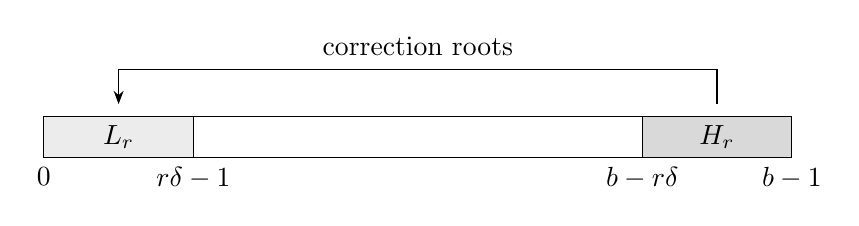
\begin{tikzpicture}[x=0.95cm,y=0.8cm,>=Stealth]
 \fill[gray!15] (0,0) rectangle (2,0.65);
 \fill[gray!30] (8,0) rectangle (10,0.65);
 \draw (0,0) rectangle (10,0.65);
 \draw (2,0)--(2,0.65) (8,0)--(8,0.65);
 \node at (1,0.325) {$L_r$};
 \node at (9,0.325) {$H_r$};
 \draw[->] (9,0.85)--(9,1.4)--(1,1.4)--(1,0.85);
 \node at (5,1.77) {correction roots};
 \node[below] at (0,0) {$0$};
 \node[below] at (2,0) {$r\delta-1$};
 \node[below] at (8,0) {$b-r\delta$};
 \node[below] at (10,0) {$b-1$};
\end{tikzpicture}
\caption{The correction strip $V_r$ goes from the right band
$H_r$ to the left band $L_r$; each band includes every outer index.
The proof shows that one truncated block factor moves each endpoint
by at most $\delta$.  The bound $b>2(m+1)\delta$ keeps the enlarged
bands disjoint throughout the collection.}
\label{fig:wrap-strip}
\end{figure}

More precisely, for $r\leq m$ we claim that
\begin{equation}\label{eq:strip-enlargement}
 D_h^{-1}V_rD_h\subseteq V_{r+1}.
\end{equation}
Fix a root of $V_r$.  The constituents of $D_h$ all have the
same outer source $i$ and outer target $j\ne i$, and inner
displacements between $0$ and $d$.  They commute with one
another.  A constituent that commutes with the initial root
also commutes with every conjugate of it by the other
constituents, and so can be omitted from this conjugation.

An interacting constituent changes the source endpoint only
when its target is the old source; the new source is at most
$d$ positions to the left.  It changes the target endpoint only
when its source is the old target; the new target is at most
$d$ positions to the right.  These statements follow directly
from the consecutive-root relations, including their reverse
order.  An opposite-root interaction cannot occur.  Initially
the source inner index minus the target inner index is greater
than $b-2r\delta$.  After one endpoint has moved, the difference
is still greater than
\[
 b-(2r+1)\delta>\delta\geq d.
\]
Thus no constituent, whose forward displacement is at most $d$,
can be opposite to either the initial root or a root obtained
after one endpoint move.

Nor can displacements accumulate repeatedly at one endpoint
during this conjugation.  A changed source has outer index $i$,
whereas every constituent has target outer index $j\ne i$;
the source cannot change again.  A changed target has outer
index $j$, whereas every constituent has source outer index
$i$; the target cannot change again.  Both endpoints may change,
but each changes at most once.  A root with both endpoints
changed has outer indices $i,j$ and commutes with every
constituent.  All roots produced lie in $V_{r+1}$, proving
\eqref{eq:strip-enlargement}.  This reasoning applies to a product
of strip roots as well.

It remains to collect the corrections without conjugating
them by one another.  Put $D_{>h}=D_{h+1}\cdots D_m$ and
$D_{>m}=1$.  The exact group identity
\[
 \prod_{h=1}^m(D_hF_h)
  =(D_1\cdots D_m)
       \prod_{h=1}^m(D_{>h}^{-1}F_hD_{>h}),
\]
where the final product is in increasing order of $h$, does this.
Every $F_h$ starts in $V_1$, and every suffix has at most $m$
factors.  By \eqref{eq:strip-enlargement}, all final corrections
belong to $V_{m+1}$.  Therefore
\[
 W_v(C_b)=W_v(S_b)u,\qquad u\in V_{m+1}.
\]
Both evaluated words have identity matrix image.  The same is
true of $u$, and the disjointness of $H_{m+1}$ and $L_{m+1}$
makes $V_{m+1}$ faithful.  Hence $u=1$.
\end{proof}

\subsection{Graded evaluation and powers of central elements}

Return to the graded algebra $R=\bigoplus_{a\geq0}R_a$ with
$R_0=\F_2$.  The map
\[
 \gamma:R\longrightarrow R[t],\qquad
       \sum_a r_a\longmapsto\sum_a r_a t^a
       \quad(r_a\in R_a)
\]
is a unital algebra homomorphism.  Applying it to a root word
representing $z\in J(R)$ gives a word $z(t)$ with identity
matrix image over $R[t]$.  Its evaluations at $1$ and $0$ are
$z$ and the degree-zero reduction of $z$, respectively.

For $T\in\Mat_b(\F_2)$, fix an injection from the pairs $(i,s)$,
where $i$ ranges over the stable index set and $0\leq s<b$,
into the stable index set.  Define $W_z(T)$ by applying the
graded substitution and evaluating by block roots in those
coordinates.  This is a homomorphism on $\St(R)$ by
Lemma~\ref{lem:block-laws}, so $W_z(T)$ depends only on $z$.
The element $W_z(T)$ belongs to $J(R)$.  All words and their
block evaluations use finitely many coordinates; choosing a
different injection gives the same element by centrality and
Lemma~\ref{lem:permutations}.

\begin{lemma}[Vanishing at long cyclic shifts]\label{lem:cyclic-vanishing}
If $z\in J(R)$ maps to $1$ in $\St(\F_2)$, then
\[
 W_z(C_b)=1
 \qquad\text{for every sufficiently large integer }b.
\]
More precisely, if the graded word $z(t)$ has $m\geq1$ factors
of degrees at most $d$, it suffices that
$b>2(m+1)\max\{1,d\}$.
\end{lemma}

\begin{proof}
Choose one finite root word for $z$, and apply
Lemma~\ref{lem:wrap} to its graded word.  Since $S_b$ is strictly
upper triangular, Lemma~\ref{lem:triangular} gives, in the stable
group,
\[
 W_z(C_b)=W_z(S_b)
       =\prod_{s=0}^{b-1}\iota_s(z(0))=1.
\]
The fixed injection extends each $\iota_s$ to a homomorphism on
the stable group.  Since $z(0)$ is trivial there by hypothesis,
every displayed coordinate image is trivial.  The empty word
satisfies the conclusion for all $b$.
\end{proof}

\begin{proposition}[Relative $2$-primary torsion]\label{prop:relative-torsion}
Every element of
\[
 J(R)\cap\ker\bigl(\St(R)\longrightarrow\St(\F_2)\bigr)
\]
has finite $2$-power order.
\end{proposition}

\begin{proof}
Let $z$ be such an element.  If $b$ is a power of two, then
$C_b^b=\Id$ and characteristic two gives
$(C_b-\Id)^b=0$.  A basis adapted to the successive kernels of
the nilpotent map $C_b-\Id$ makes $C_b$ upper triangular with
all diagonal entries $1$.  Thus some
$P\in\GL_b(\F_2)$ has this effect.  By
Lemma~\ref{lem:block-laws}, conjugation by a Steinberg lift of
the repeated basis change takes $W_z(C_b)$ to
$W_z(P^{-1}C_bP)$.  Centrality of $J(R)$ makes these elements
equal.  Lemma~\ref{lem:triangular} then gives
\begin{equation}\label{eq:cyclic-two-power}
 W_z(C_b)=\prod_{s=0}^{b-1}\iota_s(z)=z^b.
\end{equation}
The last equality uses Lemma~\ref{lem:permutations}: every
coordinate image of the central element $z$ equals $z$ in the
stable group.  Choose a power of two $b$ large enough for
Lemma~\ref{lem:cyclic-vanishing}.  Then $z^b=1$.
\end{proof}

Only the positive grading and the degree-zero field were used
in this section.  To detect central elements by finite degree
truncations, we next use the additional phase structure of the
specific algebra $R$.  It will yield an odd-power counterpart
of \eqref{eq:cyclic-two-power}.

\section{Commutators of long entries}\label{sec:long-entries}

The phase property will let us distribute a long word among several
coordinate blocks. To do this inside the Steinberg group, we must control
the extra factors produced by moving its roots. The main point of this
section is that these factors lie in an abelian subgroup on which the
matrix map is injective. Opposite roots require particular care: their
commutation cannot be inferred just from their matrix images.

Fix an odd integer $L$ and a threshold $N\ge1$ from
Lemma~\ref{lem:phases}. Let $k$ bound the lengths of the defining word
rules, and fix
\begin{equation}\label{eq:long-threshold}
 M\ge 2N+k+1.
\end{equation}
All groups in this section are stable groups over $R$. We identify a
nonzero word class with its basis element in $R$, and write $|w|$ for its
length. Write $E_{ij}$ for the matrix unit in position $(i,j)$.
Phases always take values in $\Z/L$.

\subsection{Opposite roots and movement of a cut}

\begin{lemma}\label{lem:opposite}
Suppose $a,c\in R$ satisfy $ca=0$. For distinct indices $i,h,j$ and
every $b\in R$,
\begin{equation}\label{eq:cut-movement}
 [x_{ij}(ab),x_{ji}(c)]
   =[x_{ih}(a),x_{hi}(bc)].
\end{equation}
In particular, $[x_{ij}(a),x_{ji}(c)]$ is independent of $j\ne i$.
It commutes with both defining roots, has square $1$, and has matrix
image $\Id+acE_{ii}$.
\end{lemma}

\begin{proof}
Apply Lemma~\ref{lem:commutator} to
\[
 X=x_{ih}(a),\qquad Y=x_{hj}(b),\qquad Z=x_{ji}(c).
\]
Then $A=[X,Y]=x_{ij}(ab)$ and $B'=[Y,Z]=x_{hi}(bc)$.
The Steinberg relations give $[A,X]=[B',Z]=1$.
They also give $[X,Z]=1$ because $ca=0$, and $[A,B']=1$
because $(bc)(ab)=b(ca)b=0$. This proves
\eqref{eq:cut-movement}.

Taking $b=1$ proves independence of the auxiliary index. Express the
commutator using an index $h$ different from $i,j$. Each of its two
factors then commutes with $x_{ij}(a)$ and with $x_{ji}(c)$: the only
potential nonzero consecutive-root coefficient is $ca$. Thus the
commutator commutes with both defining roots. Since each root has
square $1$, expanding $[x_{ij}(a)^2,x_{ji}(c)]$ shows
that its square is $1$. Finally, multiplication of the four elementary
matrices, using $ca=0$, gives $\Id+acE_{ii}$.
\end{proof}

\begin{lemma}\label{lem:long-commutator}
For each coordinate $i$ and every nonzero word class $w$ satisfying
$|w|\ge M$ and $\sigma(w)\ne\tau(w)$, there is an element
$H_i(w)\in\St(R)$ with the following property. If $p,q$ are nonzero
words with
\[
 |p|,|q|\ge N,\qquad |p|+|q|\ge M,
 \qquad \sigma(p)\ne\tau(q),
\]
then, for every $j\ne i$,
\begin{equation}\label{eq:long-opposite}
 [x_{ij}(p),x_{ji}(q)]
 =\begin{cases}
    H_i(w),& pq\text{ represents the nonzero class }w,\\
    1,& pq=0\text{ in }R.
   \end{cases}
\end{equation}
The element $H_i(w)$ has square $1$ and matrix image
$\Id+wE_{ii}$.
\end{lemma}

\begin{proof}
The phase mismatch gives $qp=0$, so
Lemma~\ref{lem:opposite} applies. We first show that the commutator
does not change when the cut between $p$ and $q$ moves, provided both
new parts still have length at least $N$.

For a move to the right, write the original word as $abc$, with
$a=p$ and $bc=q$, and with $|c|\ge N$. The word $c$ is nonzero and
has $\tau(c)=\tau(q)$. Hence $ca=0$, and
\eqref{eq:cut-movement}, together with auxiliary-index independence,
identifies the commutators for the cuts $a\mid bc$ and $ab\mid c$.
This equality remains valid if $ab=0$, in which case the commutator
is $1$. Otherwise $\sigma(ab)=\sigma(a)$, so the new cut retains
the mismatch. For a move to the left, write $p=ab$ and $q=c$ with
$|a|\ge N$. Now $a$ is nonzero with $\sigma(a)=\sigma(p)$, so
$ca=0$ again, and the same identity compares $ab\mid c$ with
$a\mid bc$. If the new suffix is zero we again obtain $1$;
otherwise its end phase is unchanged. This proves invariance under
every allowed movement of the cut. If a part becomes zero, the
equalities already obtained show that the original commutator was
$1$, and the argument can stop.

Next consider a single defining replacement inside a word of length
$n\ge M$. The allowed cut positions are the integers in $[N,n-N]$.
A rule of length at most $k$ can straddle at most $k-1$ of these
positions, whereas \eqref{eq:long-threshold} supplies more than $k$
allowed positions. We can therefore move the cut so that the entire
replacement lies in one part. That part has the same value in $R$
before and after the replacement. If it is nonzero, its phases are
unchanged because phases depend only on the word class. The other
part is unchanged. The commutator consequently survives the
replacement with the same value and mismatch, unless a zero part has
already proved the original commutator to be $1$.

If the concatenation is nonzero, every part of every equivalent word
is nonzero. Cut movement and the preceding replacement argument show
that the commutator depends only on the class of the concatenation.
Conversely, a nonzero class $w$ as in the statement can be cut into
two parts of lengths at least $N$. The subword assertion of
Lemma~\ref{lem:phases} makes their start and end phases
$\sigma(w)$ and $\tau(w)$, respectively. Define $H_i(w)$ by any
such cut. The independence just proved makes this definition
unambiguous.

If the concatenation represents zero, the criterion
\eqref{eq:word-zero-criterion} gives a sequence of replacements
ending at a word that contains a zero-declared subword. Follow this
sequence with the commutator. Either a part has already become zero,
or the cut can be moved once more to put the final zero-declared
subword wholly in one part. That part is zero in $R$, and the
commutator is $1$. This proves the zero case as well. The order and
matrix-image assertions now follow from
Lemma~\ref{lem:opposite}.
\end{proof}

\subsection{A subgroup detected by its matrix entries}

Let $S$ be a finite set of coordinates, with a phase
$P(i)\in\Z/L$ assigned to each $i\in S$. An entry $w$ from $i$ to
$j$ will be called \emph{consistent} if it is a nonzero word class
of length at least $M$ and
\[
 \sigma(w)=P(i),\qquad \tau(w)=P(j).
\]
We call it a \emph{wrong-row entry} if instead
\begin{equation}\label{eq:wrong-row}
 |w|\ge M,\qquad \sigma(w)\ne P(i),\qquad \tau(w)=P(j).
\end{equation}
For $i\ne j$, a wrong-row entry defines the root $x_{ij}(w)$.
For $i=j$, it defines $H_i(w)$ by
Lemma~\ref{lem:long-commutator}. Let $U(S,P)$ be the subgroup
generated by all these elements.

\begin{lemma}\label{lem:wrong-row}
The subgroup $U(S,P)$ is abelian of exponent at most $2$, and the
matrix map is injective on it. Every root with a consistent entry
normalizes $U(S,P)$.
\end{lemma}

\begin{proof}
Write $U=U(S,P)$. First consider an off-diagonal generator
$x_{ij}(a)$ of $U$ and an off-diagonal root $x_{ef}(b)$ whose entry
is either wrong-row or consistent. If $j=e$ and $i\ne f$, their
commutator is $x_{if}(ab)$. The product is zero when $b$ is
wrong-row, since $\tau(a)=P(j)\ne\sigma(b)$. When $b$ is
consistent and $ab\ne0$, the product inherits $\sigma(a)$ and
$\tau(b)$, so it is a wrong-row entry from $i$ to $f$.
If $i=f$ and $j\ne e$, the reverse product $ba$ is zero, because
$\tau(b)=P(i)\ne\sigma(a)$, and the roots commute.

If the two positions are opposite, so that $e=j$ and $f=i$, the
same mismatch $\sigma(a)\ne\tau(b)$ allows us to use
\eqref{eq:long-opposite}. The commutator is $H_i(ab)$ when
$ab\ne0$, and is $1$ when $ab=0$. In the first case $ab$ is a
wrong-row entry from $i$ to itself. In particular the commutator is
$1$ whenever $b$ is wrong-row. All remaining pairs of positions
commute by the defining Steinberg relations. This proves both the
required commutations between off-diagonal generators of $U$ and
their required behavior under consistent roots.

Now take a diagonal generator $H_i(w)$. Represent it as a
commutator through an auxiliary coordinate $h\notin S$. To compare
it with a root $x_{ef}(b)$ on $S$, choose $h$ outside its indices
as well. If neither index is $i$, the supports are disjoint and the
elements commute. If one index is $i$, the root lies in a strip
between $\{i,h\}$ and its complement. By
Lemma~\ref{lem:strip}, conjugation by $H_i(w)$ acts on that strip
by its matrix $\Id+wE_{ii}$. This matrix is its own inverse,
since $w^2=0$ by the phase mismatch. Consequently, for $f\ne i$
and $e\ne i$,
\begin{align*}
 H_i(w)x_{if}(b)H_i(w)^{-1}&=x_{if}(b+wb),\\
 H_i(w)x_{ei}(b)H_i(w)^{-1}&=x_{ei}(b+bw).
\end{align*}
The incoming product $bw$ is always zero, because
$\tau(b)=P(i)\ne\sigma(w)$. The outgoing product $wb$ is zero
when $b$ is wrong-row; when $b$ is consistent and $wb\ne0$, it is
a wrong-row entry from $i$ to $f$. These formulas prove that
diagonal generators commute with off-diagonal generators of $U$,
and that their commutators with consistent roots belong to $U$.

Two diagonal generators at different coordinates can be represented
using disjoint pairs of coordinates, and hence commute. For two at
the same coordinate $i$, write the second as
\[
 H_i(w')=[x_{it}(a),x_{ti}(c)],\qquad ac=w',\quad |a|,|c|\ge N,
\]
using $t$ distinct from the auxiliary coordinate for the first.
Here $\sigma(a)=\sigma(w')\ne P(i)$ and
$\tau(c)=\tau(w')=P(i)$. The phase rule therefore gives
$wa=0$ and $cw=0$. Applying the same strip action to the two
displayed factors shows that $H_i(w)$ fixes both, and thus commutes
with $H_i(w')$. The use of parts of length at least $N$ is sufficient
for these two applications of the phase rule.

We have proved that all generators of $U$ commute. They have square
$1$ by root addition and Lemma~\ref{lem:long-commutator}. Their
matrix images are $\Id+wE_{ij}$, indexed by positions and nonzero
word classes satisfying \eqref{eq:wrong-row}. Any two added matrices
multiply to zero: a potentially nonzero product requires matching
positions, and then the end phase of the first entry is the designated
row phase of the second, which differs from its start phase. Thus a
product of distinct generators has matrix image
\[
 \Id+\sum_{(i,j,w)}wE_{ij}.
\]
The word classes form a basis of $R$, so this is the identity only
when the sum is empty. This proves injectivity on $U$.
Finally, the commutator calculations show that conjugation by any
consistent root sends every generator of $U$ into $U$. Such a root
is its own inverse, so it normalizes $U$.
\end{proof}

\section{Detection by degree truncations}\label{sec:detection}

We now show that degree truncations detect every element of $\St(R)$.
The central kernel is the essential case. For a representative whose
entries are sufficiently long, phases turn cyclic-shift evaluation
into an odd power of the original element. For an element invisible
in all truncations, Lemma~\ref{lem:cyclic-vanishing} makes the same
evaluation trivial. Its already established $2$-power order then
forces the element itself to be trivial.

Keep $L,N,M$ as in Section~\ref{sec:long-entries}. For a root word
with entries of lengths at least $M$, the following lemma puts the
start and end phases directly into the coordinate labels.

\begin{lemma}[Relocation by phases]\label{lem:relocation}
Suppose $z\in J(R)$ is represented by a finite word
\begin{equation}\label{eq:high-word}
 z=\prod_{\nu=1}^m x_{i_\nu j_\nu}(w_\nu),
 \qquad |w_\nu|\ge M,
\end{equation}
where every $w_\nu$ is a nonzero word class. Label new coordinates
by $(i,s)$, with $s\in\Z/L$. In the stable group,
\begin{equation}\label{eq:relocation}
 z=\prod_{\nu=1}^m
 x_{(i_\nu,\sigma(w_\nu)),(j_\nu,\tau(w_\nu))}(w_\nu).
\end{equation}
\end{lemma}

\begin{proof}
The empty word presents no issue, so assume $m\ge1$, and let $S$
contain the finitely many original indices and at least three
coordinates. Put
$A=\F_2\oplus R_{\ge M}\subseteq R$.
We shall compare several evaluations of the word
\eqref{eq:high-word}. Choose numerical columns
$u_s\in\F_2^L$ and rows $v_s\in(\F_2^L)^*$ such that
$v_su_s=1$ for every $s\in\Z/L$. On the word basis of the tail,
set
\begin{equation}\label{eq:phase-rank-one}
 \rho(w)=u_{\sigma(w)}v_{\tau(w)}\,w,
 \qquad \rho(1)=\Id_L,
\end{equation}
and extend linearly to $A$.
This is a unital algebra homomorphism $A\to\Mat_L(R)$.
Indeed, a nonzero product $ww'$ has matching middle phases and
inherits the outside phases, so
\[
 \rho(w)\rho(w')
 =u_{\sigma(w)}
   \bigl(v_{\tau(w)}u_{\sigma(w')}\bigr)
   v_{\tau(w')}ww'
 =\rho(ww').
\]
If $ww'=0$, the product of the two entry matrices is zero as well,
regardless of the middle numerical pairing. Scalar products are
immediate.

Applying $\rho$ to the entries in \eqref{eq:high-word}, and then
using the block roots of Lemma~\ref{lem:block-laws}, produces an
element of $J(R)$. To justify this assertion, the original matrix
word is the identity already over the subalgebra $A$, since all its
entries belong to $A$ and $A\hookrightarrow R$ is injective. Its
image under $\rho$ is therefore the identity matrix. This uses only
the matrix identity; no injectivity assertion about
$\St(A)\to\St(R)$ is needed.

Write $\mathbf e_s$ for the standard numerical columns and
$\mathbf e_s^*$ for their rows. Start with
$u_s=\mathbf e_0$ and $v_s=\mathbf e_0^*$ for every $s$.
The evaluated word is $z$ supported on the coordinates $(i,0)$,
which is the same stable element by
Lemma~\ref{lem:permutations} and centrality. We change this
evaluation in three steps.

\emph{Add entries in unused columns.}
Keep all $u_s=\mathbf e_0$, and change the rows to
\[
 v_0=\mathbf e_0^*,\qquad
 v_t=\mathbf e_0^*+\mathbf e_t^*\quad(t\ne0).
\]
Every pairing $v_tu_s$ is still $1$.
Each block root acquires at most one additional factor, going
from a coordinate $(i,0)$ to an unused coordinate $(j,t)$ with
$t\ne0$. These factors belong to the strip from
$S\times\{0\}$ to $S\times(\Z/L\setminus\{0\})$.
The original factors, supported on $S\times\{0\}$, normalize this
strip by Lemma~\ref{lem:strip}. We can therefore collect the
additional factors into a single strip element. Both the old and
new evaluated words have identity matrix image, so that strip
element has identity matrix image. Strip injectivity makes it
trivial. The new evaluation is still $z$.

\emph{Change the numerical basis.}
The rows $v_t$ just defined form a basis. Let $Q$ be the numerical
matrix with these rows, so that $v_tQ^{-1}=\mathbf e_t^*$.
Also $Q\mathbf e_0=\sum_s\mathbf e_s$, because
$v_t\mathbf e_0=1$ for every $t$. Conjugating all entry matrices
by $Q$ therefore changes the columns and rows to
\[
 u_s=\sum_{r\in\Z/L}\mathbf e_r\quad\text{for every }s,
 \qquad v_t=\mathbf e_t^*.
\]
Apply the exact block-conjugation assertion of
Lemma~\ref{lem:block-laws} with $P=Q^{-1}$. This simultaneous
basis change is induced by conjugation in $\St(R)$.
The evaluated word belongs to
the central kernel, so it remains $z$.

\emph{Remove the factors in the wrong rows.}
Give coordinate $(i,s)$ the designated phase $P((i,s))=s$.
A block root with entry $w$ now factors as
\[
 \prod_{r\in\Z/L}x_{(i,r),(j,\tau(w))}(w).
\]
Its factors commute. The factor with $r=\sigma(w)$ is the root
in \eqref{eq:relocation}; all the other factors are wrong-row
generators of $U(S\times\Z/L,P)$.
Lemma~\ref{lem:wrong-row} says that the retained, consistent roots
normalize this subgroup. Collecting the other factors expresses
the evaluated word as the right side of \eqref{eq:relocation}
times an element $u\in U(S\times\Z/L,P)$.
The retained word itself has identity matrix image: apply
\eqref{eq:phase-rank-one} with
$u_s=\mathbf e_s$ and $v_t=\mathbf e_t^*$.
Hence $u$ has identity matrix image. Injectivity on the wrong-row
subgroup gives $u=1$, proving \eqref{eq:relocation}.
\end{proof}

\begin{proposition}\label{prop:odd-power}
Under the hypotheses of Lemma~\ref{lem:relocation},
\begin{equation}\label{eq:odd-power}
 W_z(C_L)=z^L.
\end{equation}
\end{proposition}

\begin{proof}
For a homogeneous word $w$ of degree $d=|w|$, the cyclic-shift
evaluation of $x_{ij}(w)$ is the block root with entry $wC_L^d$.
Since $\tau(w)-\sigma(w)=d$ in $\Z/L$, its factors are
\begin{equation}\label{eq:offset-factors}
 x_{(i,\sigma(w)+a),(j,\tau(w)+a)}(w),
 \qquad a\in\Z/L.
\end{equation}
We claim that any two such factors arising from different offsets
$a\ne a'$ commute, even when they come from different roots of the
original word.

Write their entries as $w,w'$. A match between the column coordinate
of the first factor and the row coordinate of the second requires
$\tau(w)+a=\sigma(w')+a'$. Since $a\ne a'$, this implies
$\tau(w)\ne\sigma(w')$, and hence $ww'=0$.
A match in the reverse direction similarly implies $w'w=0$.
Thus the Steinberg relations prove the claim unless the two roots
are opposite. In that case both products vanish, and the reverse
match also gives $\sigma(w)\ne\tau(w')$.
Lemma~\ref{lem:long-commutator}, whose length hypotheses hold
because $|w|,|w'|\ge M\ge N$, then gives
$[x_{uv}(w),x_{vu}(w')]=1$. This proves the claim in every case.

We may consequently collect the product by offsets, preserving
within each offset the order of the original word. The offset-zero
word is precisely the relocated word of
Lemma~\ref{lem:relocation}, and every other offset word is its
coordinate permutation. They all give $z$, since $z\in J(R)$.
There are $L$ offsets, proving \eqref{eq:odd-power}.
\end{proof}

It remains to obtain a long-entry representative from triviality in
a degree truncation. Stable coordinates make this possible: a spare
coordinate separates the two factors of a long word while it is
being conjugated.

\begin{lemma}\label{lem:high-entries}
For every integer $M\ge1$, each element of
\[
 \ker\bigl(\St(R)\longrightarrow\St(R/R_{\ge2M})\bigr)
\]
can be represented by a finite product of roots whose entries are
nonzero word classes of lengths at least $M$.
\end{lemma}

\begin{proof}
For any two-sided ideal $K$ of a unital ring, the Steinberg
presentation shows that the kernel of
$\St(R)\to\St(R/K)$ is the normal closure of the roots
$x_{ij}(a)$ with $a\in K$. Indeed, after these roots are killed,
root addition makes $x_{ij}(a)$ depend only on the class of $a$
modulo $K$, and the remaining relations are exactly the
Steinberg relations over $R/K$.
For $K=R_{\ge2M}$, root addition expands every such entry in the
homogeneous word basis. It is therefore enough to handle a
conjugate $g x_{ij}(w)g^{-1}$ with $|w|\ge2M$.

Choose a representative word $w=ab$ with $|a|,|b|\ge M$.
Both parts are nonzero because $w$ is nonzero. Let $S$ contain
$i,j$ and every coordinate used by a fixed root word for $g$,
and choose $h\notin S$. The consecutive-root relation gives
\[
 g x_{ij}(w)g^{-1}
   =[g x_{ih}(a)g^{-1},\,g x_{hj}(b)g^{-1}].
\]
The two conjugated factors lie respectively in the strips from
$S$ to $\{h\}$ and from $\{h\}$ to $S$.
More explicitly, write $A_g=\pi(g)|_S$. By Lemma~\ref{lem:strip},
\begin{align*}
 g x_{ih}(a)g^{-1}
   &=\prod_{r\in S}x_{rh}\bigl((A_g)_{ri}a\bigr),\\
 g x_{hj}(b)g^{-1}
   &=\prod_{s\in S}x_{hs}\bigl(b(A_g^{-1})_{js}\bigr).
\end{align*}
Since $R_{\ge M}$ is a two-sided ideal, every displayed entry
still belongs to $R_{\ge M}$.
Expand the two strip elements into roots, expand each entry in the
word basis, and then expand their commutator. All resulting root
entries have length at least $M$. Doing this for the finitely many
conjugates in a normal-closure expression proves the lemma.
\end{proof}

\begin{theorem}\label{thm:detection}
Degree truncations detect the stable Steinberg group:
\begin{equation}\label{eq:stable-detection}
 \bigcap_{d\ge1}
 \ker\bigl(\St(R)\longrightarrow\St(R/R_{\ge d})\bigr)=1.
\end{equation}
\end{theorem}

\begin{proof}
Let $z$ lie in the displayed intersection. Its matrix image becomes
the identity modulo every $R_{\ge d}$. The grading has
$\bigcap_dR_{\ge d}=0$, so its matrix image is the identity over
$R$ and $z\in J(R)$. Taking $d=1$ also shows that $z$ maps to $1$
in $\St(\F_2)$.

By Lemma~\ref{lem:cyclic-vanishing}, $W_z(C_b)=1$ for every
sufficiently large integer $b$. Choose an odd phase modulus $L$
from Lemma~\ref{lem:phases} beyond this threshold. This choice uses
a fixed representative of $z$ and precedes every choice of a
long-entry representative. Now choose its phase threshold $N$ and
an integer $M\ge2N+k+1$.

The element $z$ is trivial in the truncation at degree $2M$.
Lemma~\ref{lem:high-entries} supplies a representative with
nonzero word entries of lengths at least $M$. Applying
Proposition~\ref{prop:odd-power} to this representative yields
\[
 z^L=W_z(C_L)=1.
\]
On the other hand, Proposition~\ref{prop:relative-torsion} gives
$z^{2^a}=1$ for some $a\ge0$, since $z\in J(R)$ has trivial
reduction to $\St(\F_2)$. The integers $L$ and $2^a$ are coprime.
Thus $z=1$.
\end{proof}

\section{Integral stability in a fixed number of coordinates}
\label{sec:stability}

The detection argument used additional coordinates in the stable
Steinberg group. To apply Theorem~\ref{thm:detection} to a finitely
presented group, we must now show that adjoining these coordinates
does not kill an element already in a fixed rank. We prove that rank
twelve suffices. All homology in this section has integral coefficients.

Throughout this Section, let $B=\F_2\oplus I_B$ be a unital associative
algebra, with $I_B$ a two-sided ideal such that every finite square
matrix over $I_B$ is nilpotent. No grading or finite generation
assumption is needed. We often suppress $B$ from the notation for its
matrix and Steinberg groups.

\begin{proposition}[Finite-rank inputs]\label{prop:finite-rank-input}
For such an algebra $B$, the following statements hold.
\begin{enumerate}[label=\textup{(\roman*)}]
\item Every tuple of columns of $B^m$ with linearly independent
reductions in $\F_2^m$ extends to an invertible matrix.
\item The kernel $J_r(B)$ is central in $\St_r(B)$ for $r\geq6$.
\item For $r\geq5$, the group $\E_r(B)$ is normal in $\GL_r(B)$,
and the natural maps
\[
 \GL_r(B)/\E_r(B)\longrightarrow
 \GL_{r+1}(B)/\E_{r+1}(B)
\]
are isomorphisms.
\end{enumerate}
\end{proposition}

These are, respectively, Lemma~5.1, Proposition~5.4, and Lemma~5.5
of the companion paper~\cite{Companion}. They have exactly the
hypotheses stated above. The integral conclusion we need is the
following.

\begin{theorem}\label{thm:stability}
Let $B=\F_2\oplus I_B$ satisfy the hypotheses of
Proposition~\ref{prop:finite-rank-input}. For every $n\geq12$, the
standard stabilization map $J_n(B)\to J_{n+1}(B)$ is an isomorphism,
and the natural homomorphism
\[
 \St_n(B)\longrightarrow\St(B)
\]
is injective.
\end{theorem}

The ring $B$ is local: its elements outside $I_B$ are units, whereas
its elements in $I_B$ are nilpotent. Thus the injectivity conclusion
also follows, with a better rank bound, from the classical stability
theorem of Suslin and Tulenbaev~\cite[Theorem~4.1]{SuslinTulenbaev1976}.
We include a direct proof to make the integral homology comparison
and its natural maps explicit. It compares successive ranks by the
action on ordered frames, following the classical method of
homological stability for linear groups; see
van der Kallen~\cite{vanderKallen1980}.
Two details matter here: we use ordered frames with integral chains,
and identify the second homology of their stabilizers by universal
central extensions. We give both arguments explicitly.

\subsection{Central extensions of frame stabilizers}

A group is \emph{perfect} if it equals its commutator subgroup.
A \emph{universal central extension} of a perfect group $H$ is a central
extension $\widetilde H\to H$ admitting a unique homomorphism over $H$
to every central extension of $H$. Its kernel is naturally
$H_2(H;\Z)$; this identification is natural for homomorphisms lifted
between universal central extensions. We use this standard connection
between Steinberg groups and second homology in its integral form;
see~\cite[Theorems~III.5.4 and III.5.5]{WeibelK}.

For $r\geq6$ and $l\geq0$, put
\begin{equation}\label{eq:frame-stabilizer}
 S_{r,l}=
 \left\{\begin{pmatrix}A&0\\ C&\Id_l\end{pmatrix}:
 A\in\E_r(B),\ C\in\Mat_{l\times r}(B)\right\}.
\end{equation}
This is the semidirect product of its additive lower-left strip with
$\E_r(B)$. Replace $\E_r(B)$ in this semidirect product by
$\St_r(B)$, acting through its matrix image, and denote the resulting
group by $\widetilde S_{r,l}$. There is a natural surjection
$\widetilde S_{r,l}\to S_{r,l}$ with kernel $J_r(B)$.

\begin{lemma}\label{lem:stabilizer-uce}
The map $\widetilde S_{r,l}\to S_{r,l}$ is a universal central
extension. Consequently the inclusion of the complementary block
induces a natural isomorphism
\begin{equation}\label{eq:stabilizer-homology}
 H_2(\E_r(B);\Z)\xrightarrow{\ \sim\ }
 H_2(S_{r,l};\Z),
\end{equation}
and both groups identify naturally with $J_r(B)$.
\end{lemma}

\begin{proof}
The extension is central by
Proposition~\ref{prop:finite-rank-input}\textup{(ii)}, because its
kernel acts trivially on the strip. Both its source and target are
perfect. Indeed, an internal root is a consecutive-root commutator,
and a strip root has the same expression using an intermediate index
among the first $r$ coordinates.

Consider an arbitrary central extension $T\to S_{r,l}$. The roots
available in $S_{r,l}$ are $e_{ij}(a)$ with $j\leq r$ and
$i\ne j$, where $i$ may also be one of the last $l$ coordinates.
Choose arbitrary lifts $y_{ij}(a)\in T$. We first show that lifts of
roots appearing in a Steinberg commuting relation actually commute:
\begin{equation}\label{eq:lifts-commute}
 [y_{ij}(a),y_{kt}(b)]=1
 \qquad\text{if }j\ne k\text{ and }i\ne t.
\end{equation}
Choose $h\leq r$ distinct from $i,j,k,t$. In matrices,
\[
 e_{ij}(a)=[e_{ih}(a),e_{hj}(1)],
\]
and both factors on the right commute with $e_{kt}(b)$. In $T$,
their commutators with $y_{kt}(b)$ are therefore central. Conjugating
each factor by $y_{kt}(b)$ changes it only by a central factor, so
fixes their commutator. Since this commutator differs from
$y_{ij}(a)$ by a central element, \eqref{eq:lifts-commute} follows.
The bound $r\geq6$ supplies every spare index used below as well.

Define corrected lifts by
\begin{equation}\label{eq:canonical-root-lift}
 \widehat y_{ij}(a)=[y_{ih}(a),y_{hj}(1)],
 \qquad h\leq r,\quad h\ne i,j.
\end{equation}
They are independent of $h$ and satisfy
\begin{equation}\label{eq:lifts-product}
 [y_{ih}(a),y_{hj}(b)]=\widehat y_{ij}(ab)
 \qquad(h\leq r;\ i,h,j\text{ distinct}).
\end{equation}
To prove this, choose a fourth distinct index $f\leq r$ and apply
Lemma~\ref{lem:commutator} to
\[
 X=y_{ih}(a),\qquad Y=y_{hf}(b),\qquad Z=y_{fj}(1).
\]
All its commuting hypotheses follow from
\eqref{eq:lifts-commute}, since $[X,Y]$ and $[Y,Z]$ lift,
respectively, $e_{if}(ab)$ and $e_{hj}(b)$. The resulting identity
equates the left side of \eqref{eq:lifts-product} with
$[y_{if}(ab),y_{fj}(1)]$: replacing a lift by a central multiple does
not change a commutator. Setting $b=1$ proves independence in
\eqref{eq:canonical-root-lift}; the same identity then proves
\eqref{eq:lifts-product} for arbitrary $b$.

The corrected lifts are additive in their parameters. In
\eqref{eq:canonical-root-lift}, use
$y_{ih}(a)y_{ih}(a')$ as a lift of $e_{ih}(a+a')$ and expand its
commutator with $y_{hj}(1)$. Equation~\eqref{eq:lifts-commute}
allows the commutator factors to pass the $ih$ factors, giving
\[
 \widehat y_{ij}(a+a')=
 \widehat y_{ij}(a)\widehat y_{ij}(a').
\]
Here $\widehat y_{ij}(0)=1$, since any lift of an identity matrix
is central. Together with \eqref{eq:lifts-commute} and
\eqref{eq:lifts-product}, this proves all Steinberg relations for
the corrected lifts on the available roots.

On the first $r$ coordinates they therefore define a homomorphism
$\St_r(B)\to T$. On the strip they define a homomorphism from the
additive group $\Mat_{l\times r}(B)$ to $T$. These homomorphisms
respect the semidirect-product action: conjugation of a strip root
by an internal root is determined by a commuting relation, except
when their indices form a consecutive path, in which case it is
determined by \eqref{eq:lifts-product}. These are exactly the
matrix conjugation rules. Thus they give a homomorphism
$\widetilde S_{r,l}\to T$ over $S_{r,l}$. It is unique, since two
such homomorphisms differ by a homomorphism from the perfect group
$\widetilde S_{r,l}$ to the central, abelian kernel of $T\to S_{r,l}$.
This proves universality.

Taking $l=0$ identifies $H_2(\E_r(B);\Z)$ with $J_r(B)$.
The inclusion $\E_r(B)\to S_{r,l}$ lifts by adjoining the zero
strip and is the identity on the kernels $J_r(B)$. Naturality of
the universal central extension now proves
\eqref{eq:stabilizer-homology}.
\end{proof}

\subsection{The integral complex of ordered frames}

An \emph{ordered frame} of $B^m$ is an ordered tuple of columns
whose reductions modulo $I_B$ are linearly independent. Let $C_p(m)$
be the free abelian group on ordered frames of length $p+1$, for
$p\geq0$, with boundary the alternating sum of deletions. Set
$C_{-1}(m)=\Z$, generated by the empty frame, and augment by sending
each one-column frame to $1$. Every ordering is a separate generator;
we impose no relation that identifies two orderings by a sign.

The corresponding finite complexes are complexes of injective words
on matroid independence complexes. Their shellability is established
in~\cite[Theorem~1.2 and Example~3.3]{JonssonWelker2009}. The following
direct proof gives the precise integral vanishing range we need.

\begin{lemma}\label{lem:ordered-frames}
The augmented chain complex $C_\bullet(m)$ is exact in degrees at
most $m-2$.
\end{lemma}

\begin{proof}
First let $V$ be a finite labeled collection of nonzero vectors
spanning a vector space of dimension $m$. Different labels remain
different vertices even if their vectors agree. Write $C_\bullet(V)$
for the augmented complex on its ordered independent tuples. We prove
the claimed vanishing by induction on the number of labels, allowing
$m=0$: the empty collection has its only chain group in degree $-1$,
and the asserted range is then empty.

Delete a label $v$, and let $V'=V\setminus\{v\}$. In the relative
complex
\[
 Q_\bullet=C_\bullet(V)/C_\bullet(V'),
\]
the generators are the independent tuples containing $v$.
Filter $Q_\bullet$ increasingly by the number $a$ of labels before
$v$. Deleting $v$ is zero in the relative complex; deleting a label
before it lowers the filtration; deleting a label after it preserves
the filtration. Thus the associated graded complex for a fixed $a$
is a direct sum, over independent ordered prefixes
$(u_1,\ldots,u_a,v)$, of complexes in which only the suffix varies.

For one such prefix, project all remaining labeled vectors to the
quotient by $\langle u_1,\ldots,u_a,v\rangle$, and discard the zero
projections. The projected collection spans dimension $m-a-1$ and
has fewer labels than $V$. Its augmented ordered-tuple complex,
shifted up by $a+1$ degrees, is precisely the corresponding summand
of the associated graded complex, up to the constant boundary sign
$(-1)^{a+1}$. By induction its homology vanishes through degree
\[
 (m-a-1)-2+(a+1)=m-2.
\]
This also covers a zero-dimensional quotient: its sole homology in
degree $-1$ shifts to degree $a=m-1$, outside the asserted range.
The filtration is finite, so $H_i(Q_\bullet)=0$ for $i\leq m-2$.

If $V'$ still spans dimension $m$, induction and the long exact
sequence of the pair give the required vanishing for $V$.
Otherwise $V'$ spans dimension $m-1$, and $v$ is independent of its
entire span. Prepending $v$ to every tuple of $V'$ gives a chain
homotopy from its inclusion into $C_\bullet(V)$ to zero; in
augmented degree $-1$ it sends $1$ to $(v)$. The induced maps
$H_i(C_\bullet(V'))\to H_i(C_\bullet(V))$ are therefore zero.
They are also surjective for $i\leq m-2$, by the relative vanishing
just proved. The homology of $C_\bullet(V)$ vanishes in this range.

Finally, any cycle in $C_\bullet(m)$ uses finitely many columns.
Adjoin the standard basis columns to this finite collection. Their
reductions, with column labels retained, form a finite collection
spanning $\F_2^m$. The finite result supplies a bounding chain in
the asserted range, proving the Lemma.
\end{proof}

\subsection{Second homology in successive ranks}

\begin{proof}[Proof of Theorem~\ref{thm:stability}]
We now combine the stabilizer calculation with the ordered-frame
complex to prove Theorem~\ref{thm:stability}. Fix $m\geq13$ and let
$\E_m(B)$ act on ordered frames by left multiplication.
For frame lengths $l\leq5$, this action is transitive. To see this,
complete a given frame to an invertible matrix, placing it in the
last $l$ columns, and put $r=m-l$. By
Proposition~\ref{prop:finite-rank-input}\textup{(iii)}, the map
$\GL_r/\E_r\to\GL_m/\E_m$ is an isomorphism. Right multiplication
by a suitable complementary $\GL_r$ block therefore brings the
completion into $\E_m$ without changing its last $l$ columns.

The pointwise stabilizer of the last $l$ standard columns is exactly
$S_{m-l,l}$ from \eqref{eq:frame-stabilizer}. Indeed, its general
form has $A\in\GL_{m-l}$ and arbitrary lower-left strip. The strip
is elementary, and the injectivity of
$\GL_{m-l}/\E_{m-l}\to\GL_m/\E_m$ says that this matrix belongs
to $\E_m$ precisely when $A\in\E_{m-l}$. Write $S_l=S_{m-l,l}$
for the rest of the proof. All these complementary ranks are at
least eight, so Lemma~\ref{lem:stabilizer-uce} applies.

Take a free right $\Z[\E_m]$-resolution $P_\bullet\to\Z$ of the
trivial module and form the first-quadrant double complex
\begin{equation}\label{eq:frames-double-complex}
 D_{p,q}=P_q\otimes_{\Z[\E_m]}C_p(m),\qquad p,q\geq0.
\end{equation}
This is the usual equivariant homology double complex;
see~\cite[Chapter~VII]{Brown}.
Its total homology in degree two is $H_2(\E_m;\Z)$ via augmentation.
For completeness, adjoining the augmentation column $p=-1$ gives
the same tensor product with the augmented frame complex. Each
$P_q$ is free and hence flat, so
Lemma~\ref{lem:ordered-frames} makes the rows exact in the stated
range. The augmented total complex has zero homology in degrees
one and two. The long exact sequence separating its augmentation
column from \eqref{eq:frames-double-complex} consequently gives
the asserted isomorphism.

Take vertical homology first. For $0\leq p\leq4$, the permutation
module on ordered $(p+1)$-frames has one orbit and stabilizer
$S_{p+1}$. Shapiro's Lemma identifies the first page as
\begin{equation}\label{eq:frames-first-page}
 E^1_{p,q}=H_q(S_{p+1};\Z),\qquad 0\leq p\leq4.
\end{equation}
The first differential is the alternating sum of the face maps,
each expressed by a stabilizer inclusion and a coordinate change
that returns the remaining frame to the chosen standard frame.

The row $q=1$ is zero in these columns, because every $S_l$ is
perfect. In row $q=0$, all entries are $\Z$ and each face map is
the identity. Hence the first differential is zero for odd $p$ and
the identity for even $p$. In particular,
\begin{equation}\label{eq:vanishing-second-page}
 E^2_{1,1}=E^2_{2,1}=E^2_{2,0}=E^2_{3,0}=0.
\end{equation}

In row $q=2$, the two face maps from column one to column zero
coincide. Indeed, the inclusion $\E_{m-2}\to S_2$ induces an
isomorphism on $H_2$ by Lemma~\ref{lem:stabilizer-uce}, so it
suffices to compare the faces on this complementary block.
The first standard frame is $(e_{m-1},e_m)$. Deleting its first
column gives $e_m$. Deleting its second column gives $e_{m-1}$,
which is returned to $e_m$ by swapping the last two coordinates.
This swap is elementary in characteristic two and centralizes the
first $m-2$ coordinates. The two induced maps on that block are
therefore identical. Their alternating sum vanishes, and
\[
 E^2_{0,2}=H_2(S_1;\Z).
\]

No higher differential leaves position $(0,2)$. The only possible
incoming differentials are from $(2,1)$ on the second page and
$(3,0)$ on the third page; both vanish by
\eqref{eq:vanishing-second-page}. The other positions of total
degree two, $(1,1)$ and $(2,0)$, also vanish. The spectral sequence
thus shows that the edge map
\[
 H_2(S_1;\Z)\longrightarrow H_2(\E_m;\Z)
\]
is an isomorphism. This is the map induced by inclusion: the
zero-th column corresponds to the standard column $e_m$, and its
map into the total complex followed by augmentation is the usual
homology map for its stabilizer inclusion.

Combining with \eqref{eq:stabilizer-homology}, we have proved that
the natural stabilization map
\[
 H_2(\E_{m-1}(B);\Z)\longrightarrow H_2(\E_m(B);\Z)
\]
is an isomorphism for $m\geq13$. The natural identifications by
universal central extensions turn this into the isomorphism
$J_{m-1}(B)\to J_m(B)$.

Finally, an element killed by $\St_n(B)\to\St(B)$ already has
identity matrix image, since coordinate embeddings of matrix groups
are injective. It therefore lies in $J_n(B)$. If $n\geq12$, the
successive isomorphisms on these kernels show that it cannot become
trivial at any later rank. The stable group is the direct limit, so
this proves the injectivity asserted in
Theorem~\ref{thm:stability}.
\end{proof}

\section{The finitely presented residually finite 2-group}
\label{sec:construction}

Stable detection and the fixed-rank injectivity just proved now yield
finite quotients separating the group we will use. The ring $R$
throughout this section is the algebra of
Proposition~\ref{prop:ring-input}, with the hierarchy of
Proposition~\ref{prop:hierarchy-input}. Its finite degree quotients
will give actual finite groups separating the elements of
$\Gamma=\St_{12}(R)$.

\begin{proposition}\label{prop:finite-quotients}
For every $d\ge1$, the group $\St_{12}(R/R_{\ge d})$ is finite.
The homomorphisms
\[
 \St_{12}(R)\longrightarrow\St_{12}(R/R_{\ge d}),\qquad d\ge1,
\]
separate the elements of $\St_{12}(R)$.
\end{proposition}

\begin{proof}
Put $B_d=R/R_{\ge d}$. This ring is finite: it is the direct sum of
finitely many finite-dimensional vector spaces over $\F_2$.
Moreover $B_d=\F_2\oplus I_d$ with $I_d^d=0$, so every finite
square matrix over $I_d$ is nilpotent. The centrality assertion in
Proposition~\ref{prop:finite-rank-input} therefore applies to $B_d$.
The kernel of
\[
 \St_{12}(B_d)\longrightarrow\E_{12}(B_d)
\]
is central, and the matrix group on the right is finite. Hence the
center of $\St_{12}(B_d)$ has finite index. Schur's theorem states
that a group with center of finite index has finite derived subgroup
\cite{Schur1904}; see also \cite[Theorem~10.1.4]{Robinson1996}. Since $\St_{12}(B_d)$ is perfect, it is itself
finite.

Let $g\ne1$ in $\St_{12}(R)$. Theorem~\ref{thm:stability} makes
its image in $\St(R)$ nonidentity, and
Theorem~\ref{thm:detection} detects that image in $\St(B_d)$ for
some $d$. The natural square
\[
 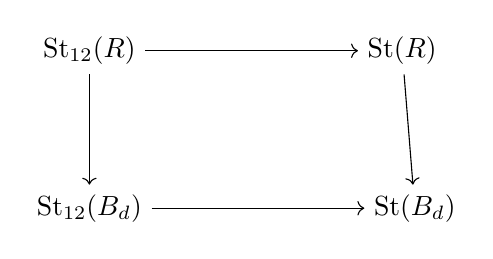
\begin{tikzpicture}[baseline=(current bounding box.center),
                    node distance=1.4cm and 2.7cm]
 \node (a) {$\St_{12}(R)$};
 \node (b) [right=of a] {$\St(R)$};
 \node (c) [below=of a] {$\St_{12}(B_d)$};
 \node (d) [right=of c] {$\St(B_d)$};
 \draw[->] (a)--(b);
 \draw[->] (a)--(c);
 \draw[->] (b)--(d);
 \draw[->] (c)--(d);
 \end{tikzpicture}
\]
commutes on each root generator. Thus the image of $g$ in
$\St_{12}(B_d)$ is nonidentity. No injectivity assertion for the
bottom arrow is needed. This proves separation by the finite groups
just constructed.
\end{proof}

\begin{proof}[Proof of Theorem~\ref{thm:main}]
The algebra $R$ is infinite and finitely presented as a unital
$\F_2$-algebra. Accordingly $\Gamma=\St_{12}(R)$ has an ordinary
finite presentation by \cite[Theorem~4.1]{Companion}; this is also a
case of \cite[Theorem~3]{KrsticMcCool}. The group $\Gamma$ is
infinite, since its matrix image contains distinct matrices
$e_{12}(a)$ for all $a\in R$. It is residually finite by
Proposition~\ref{prop:finite-quotients}.

Define
\[
 G=\ker\bigl(\Gamma\longrightarrow\St_{12}(\F_2)\bigr),
\]
where the map is induced by the degree-zero projection of $R$.
The case $d=1$ of Proposition~\ref{prop:finite-quotients} shows
that this target is finite. Thus $G$ has finite index in $\Gamma$.
It is infinite and has an ordinary finite presentation by the
Reidemeister--Schreier theorem \cite[Chapter~II, Section~4]{LyndonSchupp}. Restricting the
separating finite-quotient maps of $\Gamma$ proves residual finiteness
of $G$.

Fix $g\in G$. Its matrix image is $\Id+A$ for some
$A\in M_{12}(I)$. Proposition~\ref{prop:ring-input} gives an integer
$r\ge1$ with $A^r=0$. Choose $a\ge0$ with $2^a\ge r$.
In characteristic two,
\[
 (\Id+A)^{2^a}=\Id+A^{2^a}=\Id.
\]
Consequently $g^{2^a}\in J_{12}(R)$, and its reduction to
$\St_{12}(\F_2)$ is still trivial. Its stable image belongs to
$J(R)$ and reduces to $1$ in $\St(\F_2)$, so
Proposition~\ref{prop:relative-torsion} kills that image by a
2-power $2^b$. The injectivity in Theorem~\ref{thm:stability}
then yields $g^{2^{a+b}}=1$ in $\Gamma$, hence in $G$.
This proves every assertion of Theorem~\ref{thm:main}.
\end{proof}

\Needspace{12\baselineskip}
\begingroup\raggedright
\begin{thebibliography}{99}

\bibitem{Brown}
K.~S.~Brown,
\emph{Cohomology of Groups},
Graduate Texts in Mathematics, vol.~87,
Springer-Verlag, New York, 1982.

\bibitem{Burnside1902}
W.~Burnside,
On an unsettled question in the theory of discontinuous groups,
\emph{Quart. J. Pure Appl. Math.} \textbf{33} (1902), 230--238.

\bibitem{Golod1964}
E.~S.~Golod,
On nil-algebras and finitely approximable $p$-groups,
\emph{Izv. Akad. Nauk SSSR Ser. Mat.} \textbf{28} (1964), no.~2,
273--276 (Russian).

\bibitem{GolodShafarevich1964}
E.~S.~Golod and I.~R.~Shafarevich,
On the class field tower,
\emph{Izv. Akad. Nauk SSSR Ser. Mat.} \textbf{28} (1964), no.~2,
261--272 (Russian).

\bibitem{Grigorchuk1980}
R.~I.~Grigorchuk,
On Burnside's problem on periodic groups,
\emph{Funct. Anal. Appl.} \textbf{14} (1980), no.~1, 41--43.

\bibitem{HaettelOsajda2025}
T.~Haettel and D.~Osajda,
Locally elliptic actions, torsion groups, and nonpositively curved spaces,
arXiv:2110.12431v3 (2025).

\bibitem{JonssonWelker2009}
J.~Jonsson and V.~Welker,
Complexes of injective words and their commutation classes,
\emph{Pacific J. Math.} \textbf{243} (2009), no.~2, 313--329.

\bibitem{KrsticMcCool}
S.~Krsti\'c and J.~McCool,
Presenting $\mathrm{GL}_n(k\langle T\rangle)$,
\emph{J. Pure Appl. Algebra} \textbf{141} (1999), no.~2, 175--183.

\bibitem{LyndonSchupp}
R.~C.~Lyndon and P.~E.~Schupp,
\emph{Combinatorial Group Theory},
Ergebnisse der Mathematik und ihrer Grenzgebiete, vol.~89,
Springer-Verlag, Berlin, 1977.

\bibitem{Milnor}
J.~Milnor,
\emph{Introduction to Algebraic $K$-Theory},
Annals of Mathematics Studies, vol.~72,
Princeton University Press, Princeton, NJ, 1971.

\bibitem{NovikovAdian1968}
P.~S.~Novikov and S.~I.~Adian,
Infinite periodic groups, I--III,
\emph{Math. USSR-Izv.} \textbf{2} (1968),
209--236, 241--479, 665--685.

\bibitem{OlshanskiiSapir2003}
A.~Yu.~Ol'shanskii and M.~V.~Sapir,
Non-amenable finitely presented torsion-by-cyclic groups,
\emph{Publ. Math. Inst. Hautes \'Etudes Sci.} \textbf{96} (2003), 43--169.

\bibitem{Companion}
OpenAI,
\emph{An infinite finitely presented periodic group},
OpenAI Math Release preprint
\href{https://github.com/openai/math/blob/main/preprints/An-infinite-finitely-presented-periodic-group-September-23-2026/paper.pdf}{OAI:An-infinite-finitely-presented-periodic-group-September-23-2026},
2026.

\bibitem{Robinson1996}
D.~J.~S.~Robinson,
\emph{A Course in the Theory of Groups}, 2nd ed.,
Graduate Texts in Mathematics, vol.~80,
Springer-Verlag, New York, 1996.

\bibitem{Schur1904}
I.~Schur,
\"Uber die Darstellung der endlichen Gruppen durch gebrochen lineare
Substitutionen,
\emph{J. Reine Angew. Math.} \textbf{127} (1904), 20--50.

\bibitem{SuslinTulenbaev1976}
A.~A.~Suslin and M.~S.~Tulenbaev,
Stabilization theorem for the Milnor $K_2$-functor,
\emph{Zap. Nauchn. Sem. Leningrad. Otdel. Mat. Inst. Steklov.}
\textbf{64} (1976), 131--152 (Russian);
English translation in \emph{J. Soviet Math.} \textbf{17} (1981),
no.~2, 1804--1819.

\bibitem{vanderKallen1980}
W.~van der Kallen,
Homology stability for linear groups,
\emph{Invent. Math.} \textbf{60} (1980), no.~3, 269--295.

\bibitem{Weibel1987}
C.~A.~Weibel,
Module structures on the $K$-theory of graded rings,
\emph{J. Algebra} \textbf{105} (1987), no.~2, 465--483.

\bibitem{WeibelK}
C.~A.~Weibel,
\emph{The $K$-Book: An Introduction to Algebraic $K$-Theory},
Graduate Studies in Mathematics, vol.~145,
American Mathematical Society, Providence, RI, 2013.

\bibitem{Zelmanov1992}
E.~I.~Zel'manov,
A solution of the restricted Burnside problem for $2$-groups,
\emph{Math. USSR-Sb.} \textbf{72} (1992), no.~2, 543--565.

\end{thebibliography}

\endgroup
\end{document}
